\documentclass[10pt,a4paper,titlepage,oneside]{article}
\usepackage{LabProtocol}

\exercise{Exercise I}

% enter your data here
\authors{
	Oliver Wöhrer, Matr. Nr. 11907563 \par
	{\small e11907563@student.tuwien.ac.at} \par
}


\begin{document}

\maketitle


%████████╗ █████╗ ███████╗██╗  ██╗     ██╗
%╚══██╔══╝██╔══██╗██╔════╝██║ ██╔╝    ███║
%   ██║   ███████║███████╗█████╔╝     ╚██║
%   ██║   ██╔══██║╚════██║██╔═██╗      ██║
%   ██║   ██║  ██║███████║██║  ██╗     ██║
%   ╚═╝   ╚═╝  ╚═╝╚══════╝╚═╝  ╚═╝     ╚═╝
\Task{Structural modeling}

\begin{qa}{Create a screenshot showing the top level design in the RTL netlist viewer!}
	\begin{figure}[h!]
		\centering
		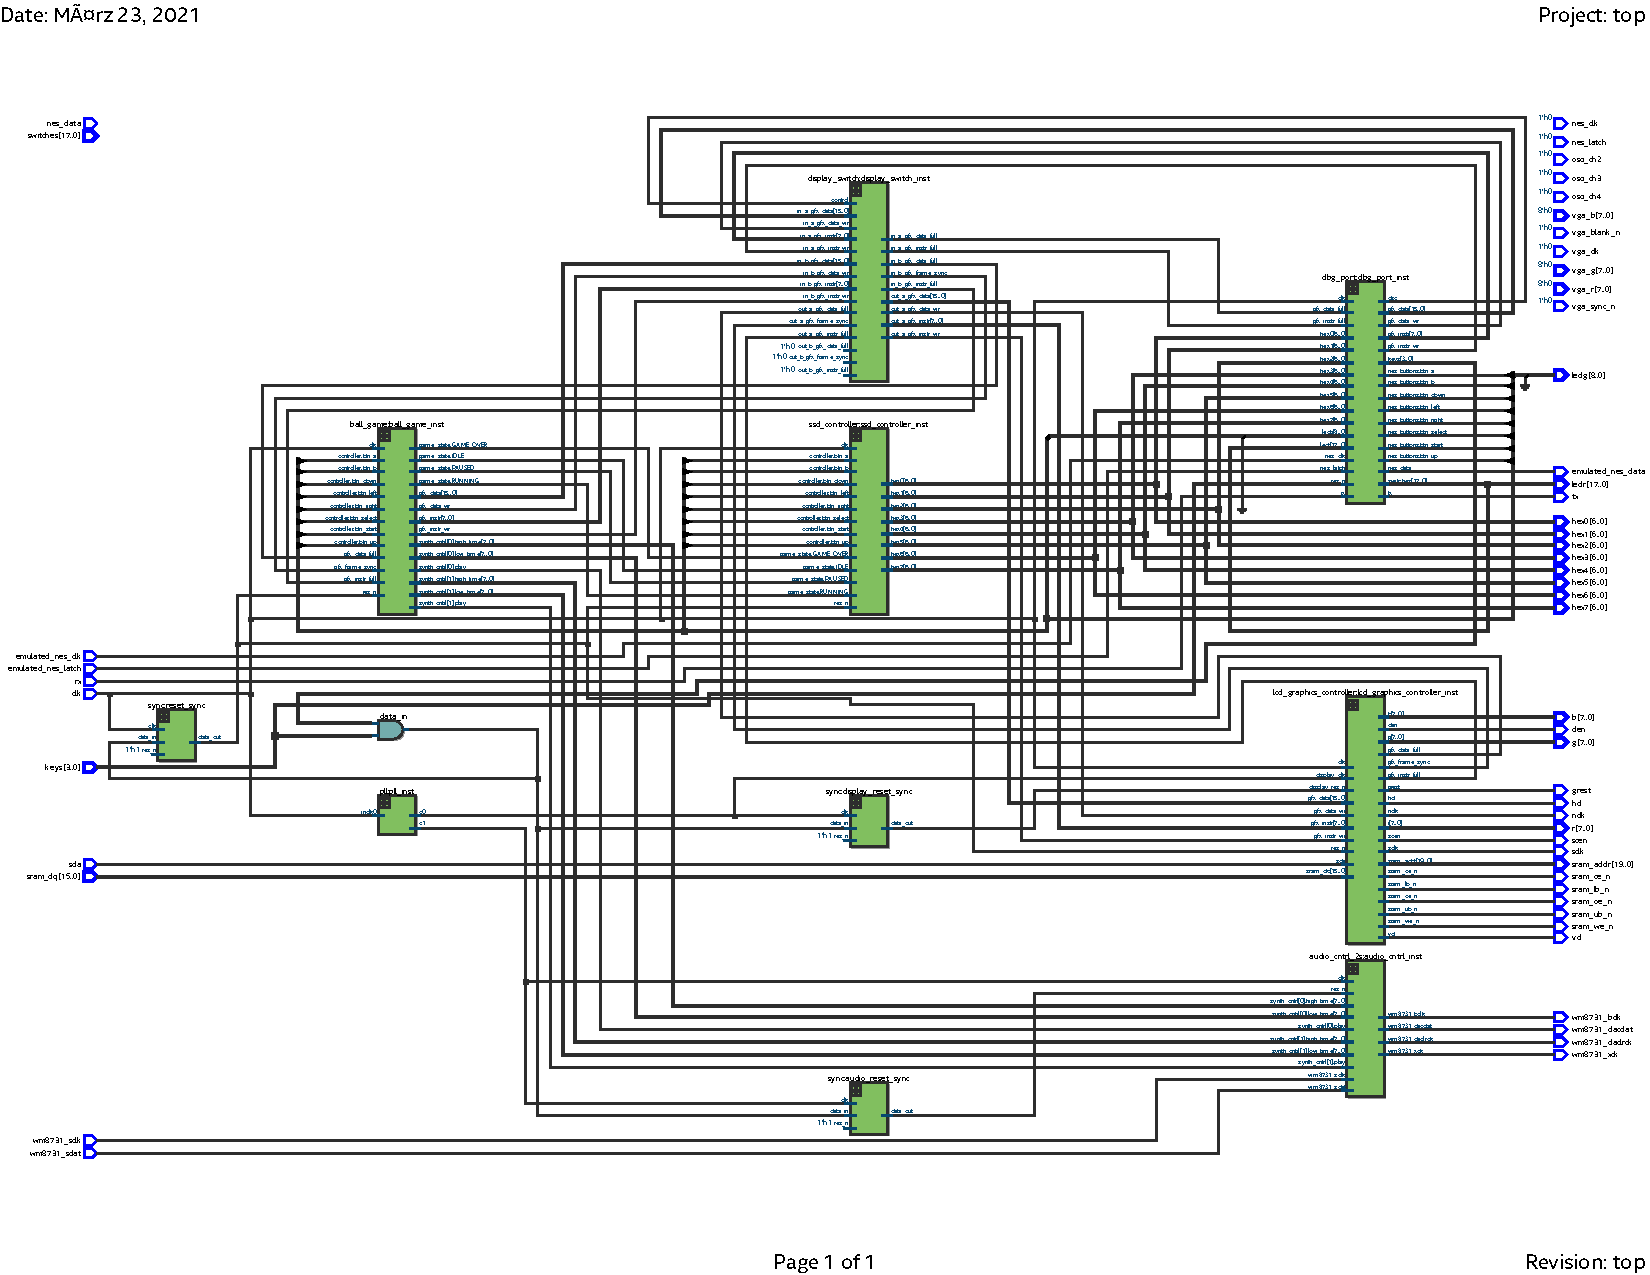
\includegraphics[width=1.0\linewidth]{dia/RTL View.pdf}
		%\dummyimage
		\caption{RTL netlist viewer screenshot}
	\end{figure}
\end{qa}
%%%%%%%%%%%%%%%%%%%%%%%%%%%%%%%%%%%%%%%%%%%%%%%%%%%%%%%%%%%%%%%%%%%%%%%%%%%%%%%%


%████████╗ █████╗ ███████╗██╗  ██╗    ██████╗ 
%╚══██╔══╝██╔══██╗██╔════╝██║ ██╔╝    ╚════██╗
%   ██║   ███████║███████╗█████╔╝      █████╔╝
%   ██║   ██╔══██║╚════██║██╔═██╗     ██╔═══╝ 
%   ██║   ██║  ██║███████║██║  ██╗    ███████╗
%   ╚═╝   ╚═╝  ╚═╝╚══════╝╚═╝  ╚═╝    ╚══════╝
\Task{Seven Segment Display I}

\begin{qa}{Are the \textsf{hex*} signals high or low-active? Explain what that means!}
According to page 36 of the user manual of the DE2-115 FPGA board used in this exercise the LEDs on the seven segment displays have an common anode. The seven segment displays therefore are low-active which means they can be driven applying a low logic level to light up the segment.\\
High-active would be the opposite, where the lights are on when the logic applied is high.
\end{qa}
%%%%%%%%%%%%%%%%%%%%%%%%%%%%%%%%%%%%%%%%%%%%%%%%%%%%%%%%%%%%%%%%%%%%%%%%%%%%%%%%

%████████╗ █████╗ ███████╗██╗  ██╗    ██████╗ 
%╚══██╔══╝██╔══██╗██╔════╝██║ ██╔╝    ╚════██╗
%   ██║   ███████║███████╗█████╔╝      █████╔╝
%   ██║   ██╔══██║╚════██║██╔═██╗      ╚═══██╗
%   ██║   ██║  ██║███████║██║  ██╗    ██████╔╝
%   ╚═╝   ╚═╝  ╚═╝╚══════╝╚═╝  ╚═╝    ╚═════╝ 
\Task{Behavioral Simulation}

\begin{qa}{SRAM write access}

\begin{center}
\begin{tabular}{lc}
	\hline
	Question & Answer \\
	\hline\hline
	Absoulte (simulation) time of the first write access$^{*}$ & 1710 ns \\
	Accessed SRAM addresses (first 4 write operations)         & 0x00, 0x01, 0x02, 0x03 \\
	Measure the SRAM timing parameter $t_{WC}$ (see datasheet) & 30 ns\\\hline
\end{tabular}

\footnotesize{$^{*}$ Take the point in time where the address for the write operation is applied.}
\end{center}

\begin{figure}[h!]
	\centering
	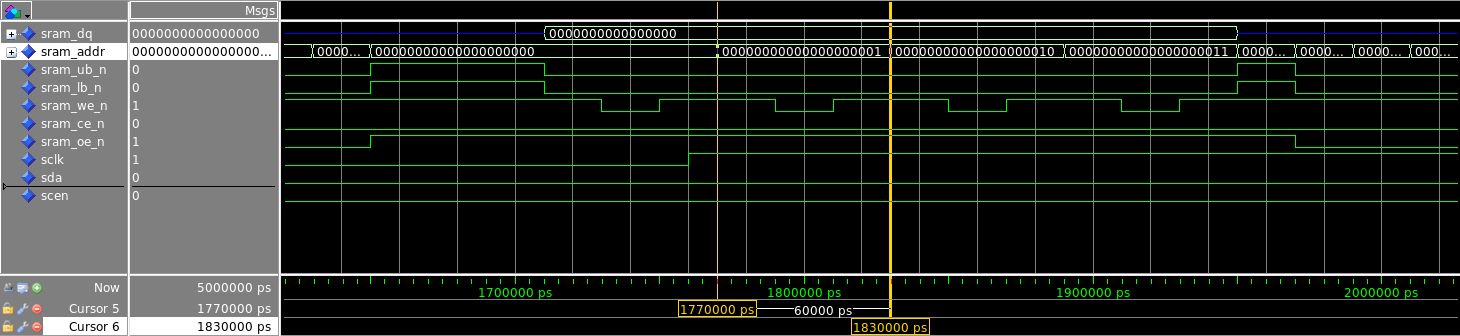
\includegraphics[width=1.0\linewidth]{dia/Subtask3.png}
	%\dummyimage
	\caption{Simulation showing the first 4 write operations to the SRAM with markers indicating the SRAM timing parameter $t_{WC}$}
\end{figure}

\end{qa}
%%%%%%%%%%%%%%%%%%%%%%%%%%%%%%%%%%%%%%%%%%%%%%%%%%%%%%%%%%%%%%%%%%%%%%%%%%%%%%%%

\begin{qa}{Serial port interface of the LCD driver IC (Consult the LCD manual to answer the following questions)}

\begin{figure}[h!]
	\centering
	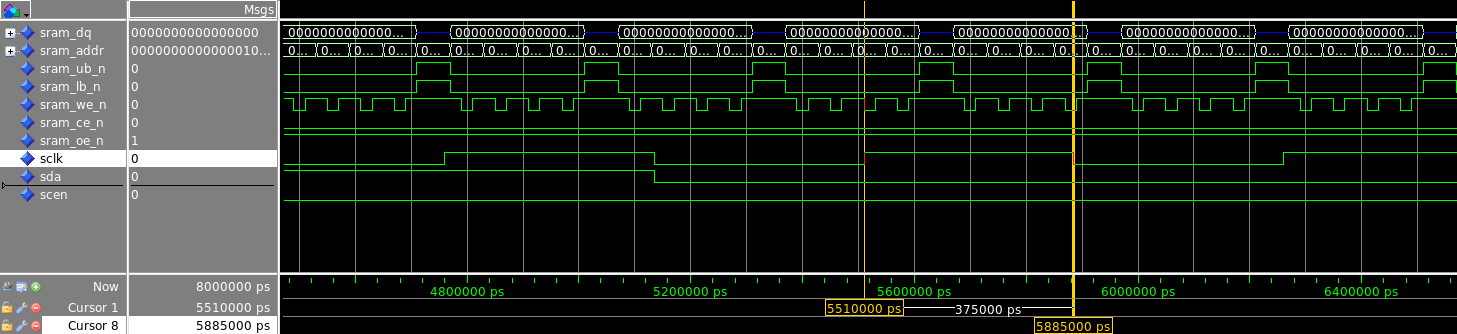
\includegraphics[width=1.0\linewidth]{dia/Subtask4.png}
	%\dummyimage
	\caption{Screenshot showing the data transmission on the serial port interface of the LCD driver IC with markers indicating the period of the $sclk$ signal.}
\end{figure}

\begin{center}
\begin{tabular}{lc}
	\hline
	Question                                               & Answer \\\hline\hline
	What frequency did you measure for the $sclk$ signal?  & 1.333 MHz \\
	What is the maximum allowed frequency?                 & 8.300 MHz \\\hline
\end{tabular}
\end{center}

Hint: Should your simulation show ``zero-width spikes'' on some signal traces, you can simply ignore them.
\end{qa}
%%%%%%%%%%%%%%%%%%%%%%%%%%%%%%%%%%%%%%%%%%%%%%%%%%%%%%%%%%%%%%%%%%%%%%%%%%%%%%%%


\begin{qa}{What is the purpose of the transmission on the serial interface to the LCD? Explain what is transmitted and why!}
The serial port interface of the LCD touch panel module is used to communicate with the LCD module and enables instruction settings. As the name suggests the data is transmitted in a serial manner. Data written to and read from the LCD is structured byte-wise and is addressed in via the number of the registers.\\
To start a data transmission the SCEN (serial clock enable pin) has to be pulled low. The address itself is five bit long and is transmitted first, followed by a R/W-bit indicating if the data is written or read at the address. After an additional 8th bit, the 8-Bit-data is transmitted MSB first.\\
After all 16 bit have been transmitted successfully all 16 rising clock edges have been detected, SCEN must go back into the logic-high state. In addition to that, the CLK goes to logic-low state in between two data transmissions.\\
\end{qa}
%%%%%%%%%%%%%%%%%%%%%%%%%%%%%%%%%%%%%%%%%%%%%%%%%%%%%%%%%%%%%%%%%%%%%%%%%%%%%%%%

%████████╗ █████╗ ███████╗██╗  ██╗    ██╗  ██╗
%╚══██╔══╝██╔══██╗██╔════╝██║ ██╔╝    ██║  ██║
%   ██║   ███████║███████╗█████╔╝     ███████║
%   ██║   ██╔══██║╚════██║██╔═██╗     ╚════██║
%   ██║   ██║  ██║███████║██║  ██╗         ██║
%   ╚═╝   ╚═╝  ╚═╝╚══════╝╚═╝  ╚═╝         ╚═╝
\Task{Postlayout Simulation}
\begin{qa}{Use a postlayout simualtion to measure the different delays on the \textsf{hex\{7-8\}} signals.}

\begin{center}
\begin{tabular}{lc}
	\hline
	Interval                                                  & Time \\ \hline\hline
	Duration between the first and the last bit toggling      &  2.529 ns \\
	Time between the last active clock edge and stabilization &  13.017 ns \\\hline
\end{tabular}
\end{center}

\begin{figure}[h!]
	\centering
	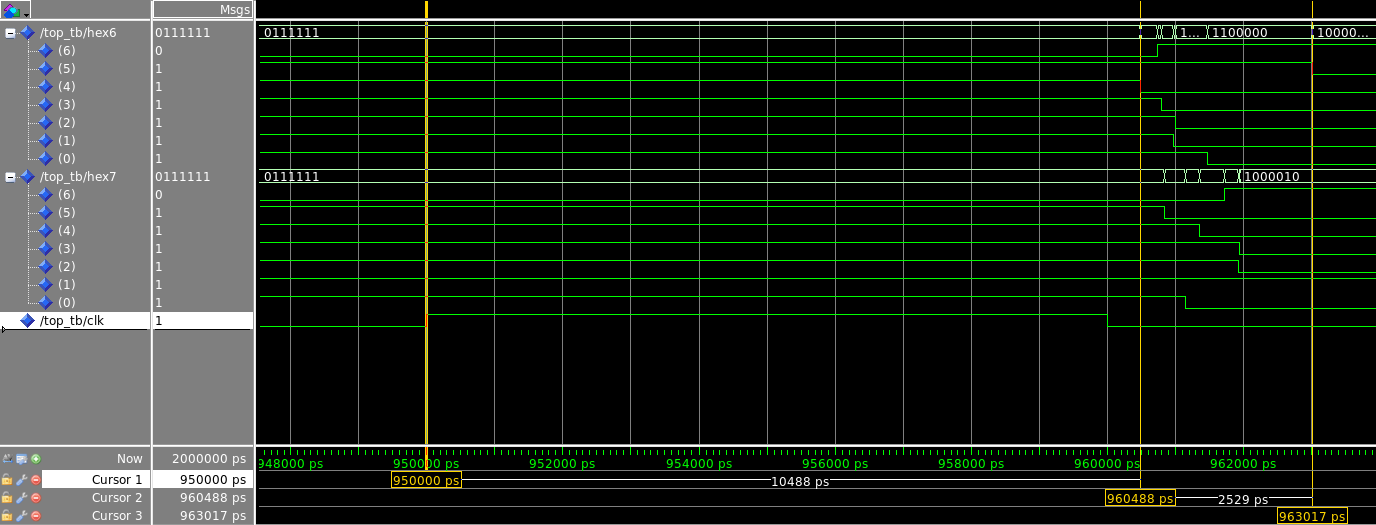
\includegraphics[width=1.0\linewidth]{dia/Subtask6.png}
	%\dummyimage
	\caption{Screenshot showing the interval measurements with markers}
\end{figure}

\end{qa}
%%%%%%%%%%%%%%%%%%%%%%%%%%%%%%%%%%%%%%%%%%%%%%%%%%%%%%%%%%%%%%%%%%%%%%%%%%%%%%%%



%████████╗ █████╗ ███████╗██╗  ██╗    ███████╗
%╚══██╔══╝██╔══██╗██╔════╝██║ ██╔╝    ██╔════╝
%   ██║   ███████║███████╗█████╔╝     ███████╗
%   ██║   ██╔══██║╚════██║██╔═██╗     ╚════██║
%   ██║   ██║  ██║███████║██║  ██╗    ███████║
%   ╚═╝   ╚═╝  ╚═╝╚══════╝╚═╝  ╚═╝    ╚══════╝
\Task{Testbench Design}

\begin{qa}{PRNG simulation}

\begin{center}
\begin{tabular}{ll}
\hline\hline
My matriculation number             & 11907563 \\
My matriculation number modulo $15$ & 8 \\
$n_a$                               & 144 \\
$n_b$                               & 159 \\
Minimum period                      & 8191 \\
Maximum period                      & 65535 \\\hline
\end{tabular}
\end{center}

\end{qa}
%%%%%%%%%%%%%%%%%%%%%%%%%%%%%%%%%%%%%%%%%%%%%%%%%%%%%%%%%%%%%%%%%%%%%%%%%%%%%%%%

\begin{qa}{Bonus Task: SRAM reads}
\begin{figure}[h!]
	\centering
	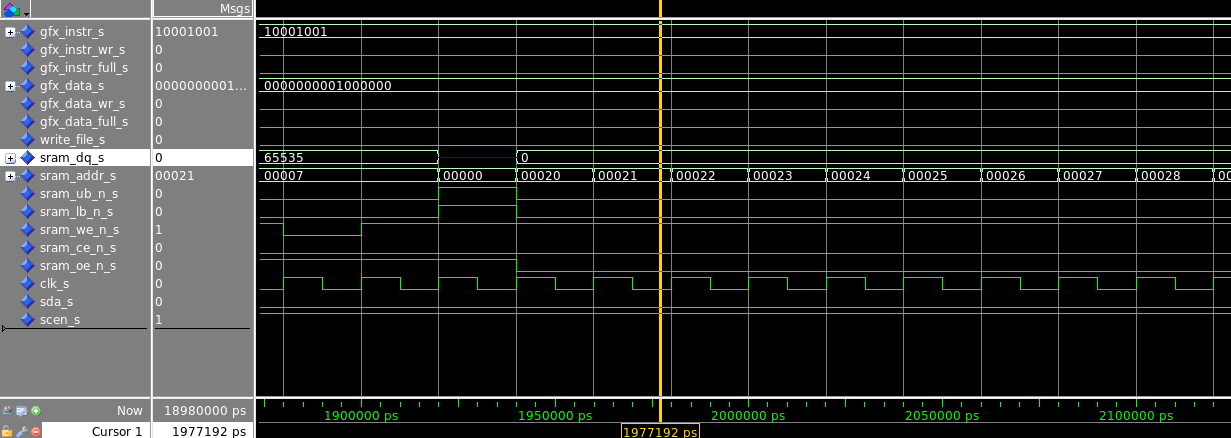
\includegraphics[width=1.0\linewidth]{dia/Subtask8.png}
	%\dummyimage
	\caption{Simulation showing a read operation performed by the \textsf{lcd\_graphics\_controller}}
\end{figure}
\end{qa}
%%%%%%%%%%%%%%%%%%%%%%%%%%%%%%%%%%%%%%%%%%%%%%%%%%%%%%%%%%%%%%%%%%%%%%%%%%%%%%%%



%████████╗ █████╗ ███████╗██╗  ██╗     ██████╗ 
%╚══██╔══╝██╔══██╗██╔════╝██║ ██╔╝    ██╔════╝ 
%   ██║   ███████║███████╗█████╔╝     ███████╗ 
%   ██║   ██╔══██║╚════██║██╔═██╗     ██╔═══██╗
%   ██║   ██║  ██║███████║██║  ██╗    ╚██████╔╝
%   ╚═╝   ╚═╝  ╚═╝╚══════╝╚═╝  ╚═╝     ╚═════╝ 
\Task{N64 Controller}

\begin{qa}{Simulation of two complete button state transmission frames}

\begin{center}
\begin{tabular}{ll}
\hline\hline
My matriculation number                   &  11907563 \\
My matriculation number modulo $2^{16}$   & 0xB1EB \\
$b_0$: hex, ({A},{B},{Select},{Start},{$\uparrow$},{$\downarrow$},{$\leftarrow$},{$\rightarrow$})  & 0xEB, (1,1,1,0,1,0,1,1) \\
$b_1$: hex, ({A},{B},{Select},{Start},{$\uparrow$},{$\downarrow$},{$\leftarrow$},{$\rightarrow$})  & 0xB1, (1,0,1,1,0,0,0,1) \\\hline
\end{tabular}
\end{center}

\begin{figure}[h!]
	\centering
	%\dummyimage
	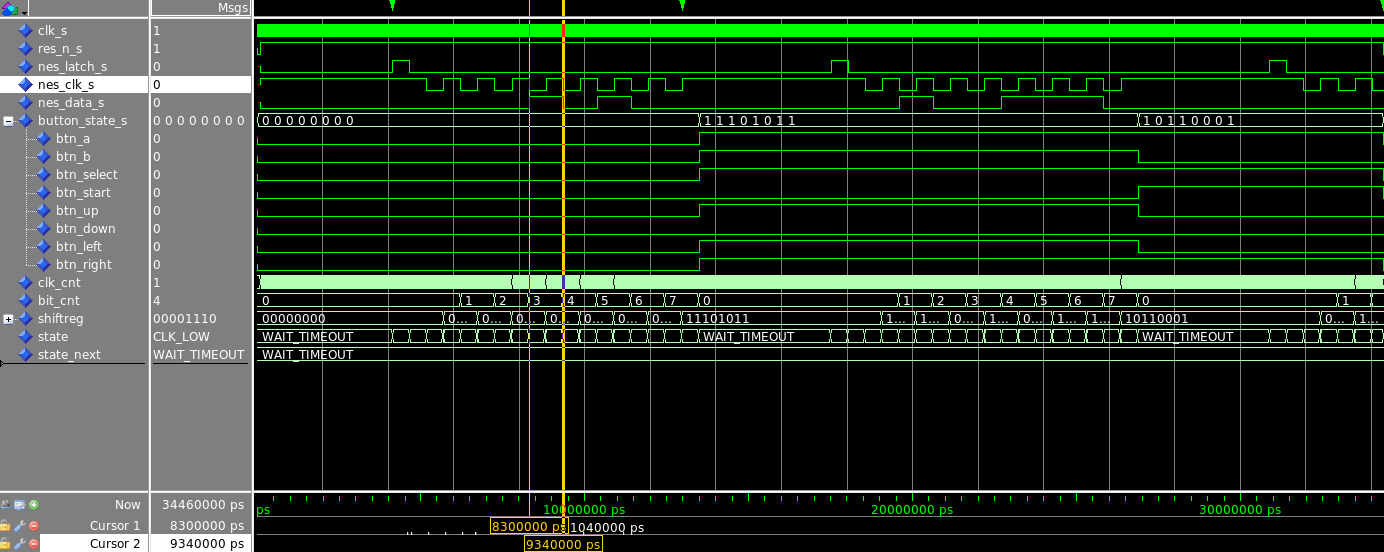
\includegraphics[width=1.0\linewidth]{dia/Subtask9.png}
	\caption{Screenshot(s) showing the both transmissions with markers shing the clock period of $nes\_clk$}
\end{figure}

\end{qa}
%%%%%%%%%%%%%%%%%%%%%%%%%%%%%%%%%%%%%%%%%%%%%%%%%%%%%%%%%%%%%%%%%%%%%%%%%%%%%%%%


\begin{qa}{Analyse the resource usage of your \textsf{nes\_controller}!}
\centering
\begin{tabular}{l|ll}
	\hline
		                       & LC Combinationals  & LC Registers  \\ \hline\hline 
	Absolute number            & 152                & 88            \\
	\% of whole design         & 4.06               & 3.57          \\ 
	\% of whole FPGA resources & 0.13               & 0.07          \\ \hline
\end{tabular}
\end{qa}
%%%%%%%%%%%%%%%%%%%%%%%%%%%%%%%%%%%%%%%%%%%%%%%%%%%%%%%%%%%%%%%%%%%%%%%%%%%%%%%%


%████████╗ █████╗ ███████╗██╗  ██╗    ███████╗
%╚══██╔══╝██╔══██╗██╔════╝██║ ██╔╝    ╚════██║
%   ██║   ███████║███████╗█████╔╝         ██╔╝
%   ██║   ██╔══██║╚════██║██╔═██╗        ██╔╝ 
%   ██║   ██║  ██║███████║██║  ██╗       ██║  
%   ╚═╝   ╚═╝  ╚═╝╚══════╝╚═╝  ╚═╝       ╚═╝  
\Task{Seven Segment Display II}

\begin{qa}{Include the state graph of the state machine you designed and briefly explain how it works.}

You can use \texttt{dia} to draw the diagram. The provided makefile automatically converts dia files to PDFs and places them in the \texttt{dia/pdf} directory.
However, any other method for drawing pictures is also fine. 

\begin{figure}[h!]
	\centering
	\includegraphics[width=0.75\linewidth]{dia/pdf/example_fsm.pdf}
	\caption{FSM state graph}
\end{figure}

\end{qa}
%%%%%%%%%%%%%%%%%%%%%%%%%%%%%%%%%%%%%%%%%%%%%%%%%%%%%%%%%%%%%%%%%%%%%%%%%%%%%%%%


\begin{qa}{Seven Segment Display Simulation Screenshot}

\begin{center}
\begin{tabular}{ll}
\hline\hline
My matriculation number                          & 11907563 \\ 
My matriculation number modulo $500$             & 63 \\ 
\textsf{player\_points} value for the testbench  & 1297 \\ \hline
\end{tabular}
\end{center}
Sub
\begin{figure}[h!]
	\centering
	For the sake of better visibility and the overall view the blink intervalls are shorten and the BLINK-INTERVAL generic is set to 6 for the first screenshot. See the other following screenshots for a more detailed wave view on the conversion procedure.
	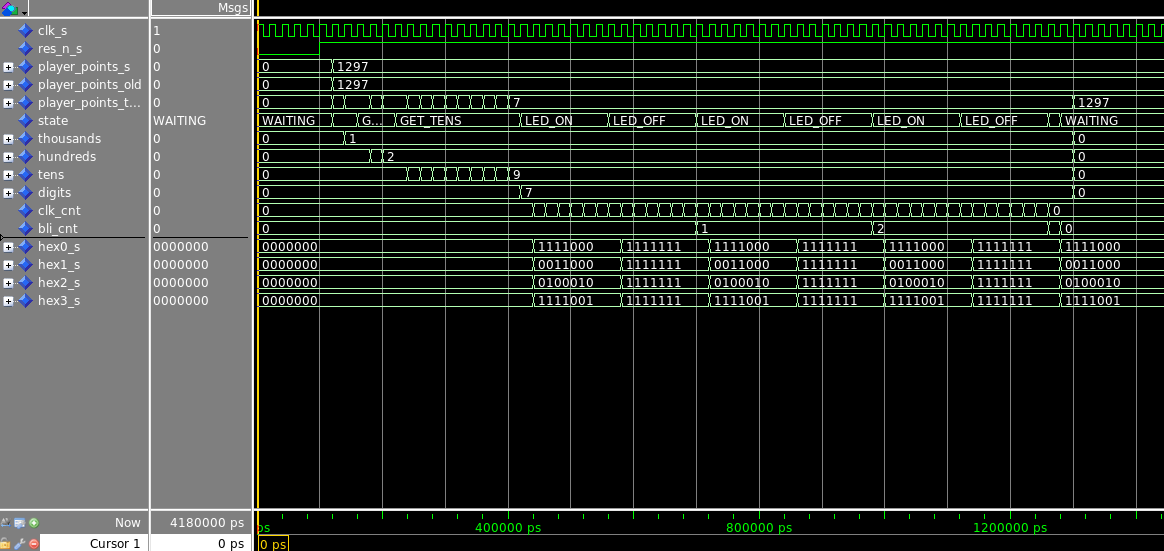
\includegraphics[width=1.0\linewidth]{dia/Subtask12_1.png}
	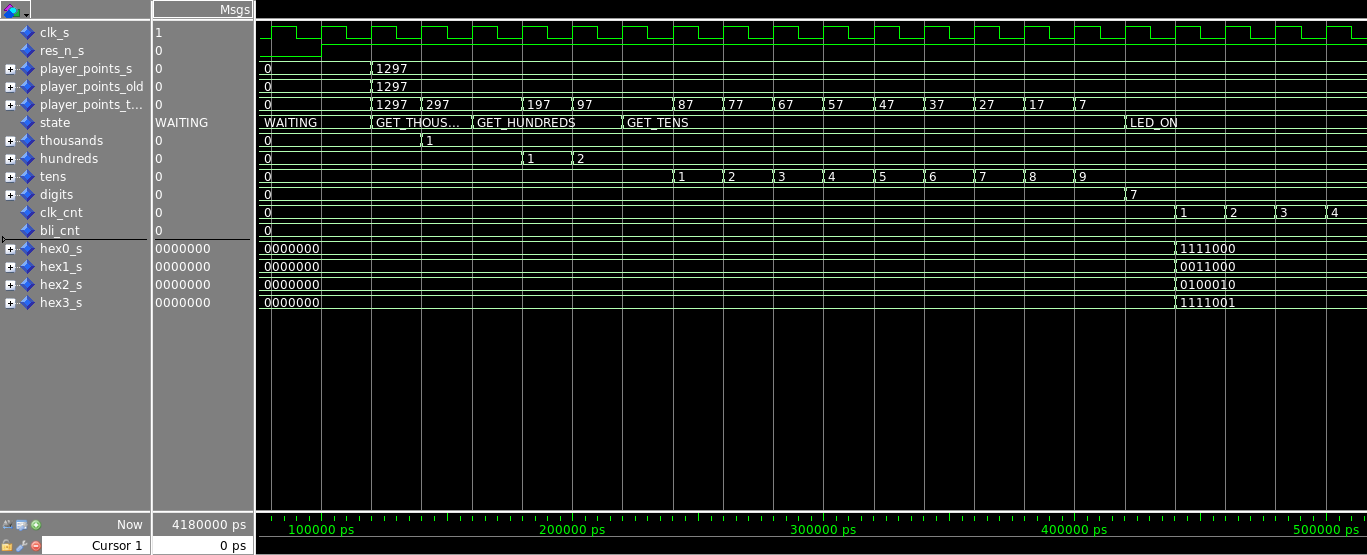
\includegraphics[width=1.0\linewidth]{dia/Subtask12_2.png}
	%\dummyimage
	\caption{Simulation showing the conversion}
\end{figure}

\end{qa}
%%%%%%%%%%%%%%%%%%%%%%%%%%%%%%%%%%%%%%%%%%%%%%%%%%%%%%%%%%%%%%%%%%%%%%%%%%%%%%%%

\begin{qa}{Bonus Task: Animation Simulation}
\begin{figure}[h!]
	\centering
	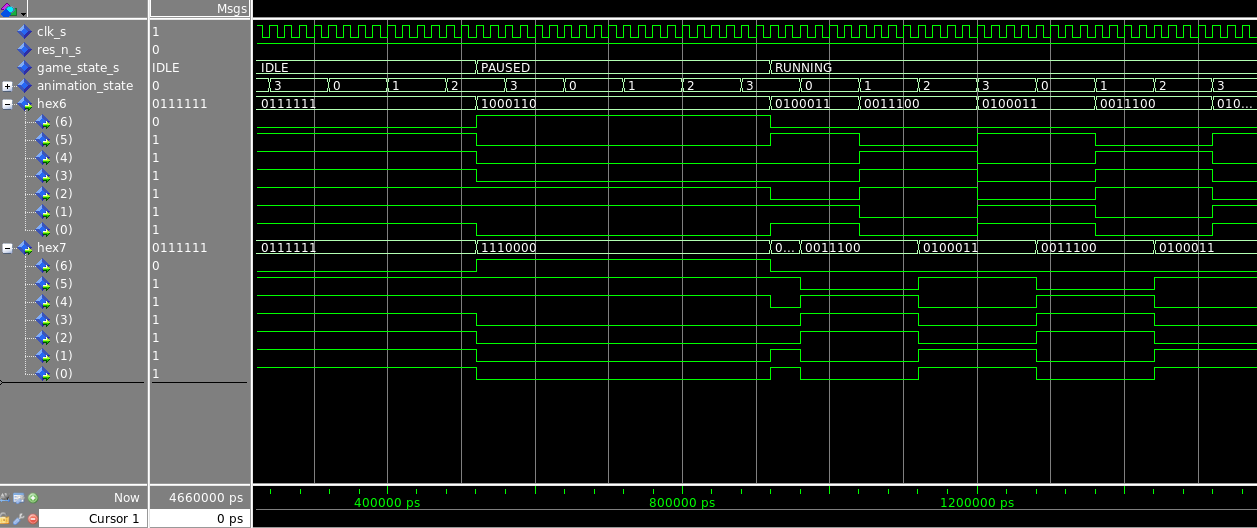
\includegraphics[width=1.0\linewidth]{dia/Subtask13.png}
	%\dummyimage
	\caption{Simulation showing all animation steps}
\end{figure}
\end{qa}
%%%%%%%%%%%%%%%%%%%%%%%%%%%%%%%%%%%%%%%%%%%%%%%%%%%%%%%%%%%%%%%%%%%%%%%%%%%%%%%%


\end{document}

